\chapter{Wi-Fi Technology}
\label{chap:wifi}
This chapter provides background information to understand the essentials about the traffic sent on a Wi-Fi network, architecture of the designed system and background behind the KRACK attacks principle. First, we describe general technical information about Wi-Fi network and standards which define it. Then, we talk about the structure of the frames sent on such a system. This part is necessary to understand both regular traffic and the one generated during the attack. The association and authentication on a Wi-Fi network are after that explained along with the handshakes vulnerable to the KRACK attacks.  

Wi-Fi is a trademark for a wireless network technology based on the IEEE~802.11 family of standards. As the name implies, these standards were made by the \gls{ieee}. IEEE~802 refers to a family of IEEE standards dealing with a \gls{lan} and a \gls{man}. This family is maintained by the \gls{lmsc}. An individual \gls{wg} provides the focus for each area (for example, 802.3 Ethernet, 802.15.1 Bluetooth, and 802.16 WiMAX, etc.). IEEE~802.11 family of standards deals with the implementation of the \gls{wlan}.

The services and protocols specified in IEEE~802 target \gls{dll} and \gls{phy}, the lowest two layers of the seven-layer OSI networking reference model. IEEE~802 splits the OSI Data Link Layer into two sublayers,  \gls{llc} and \gls{mac}. The layers structure is shown in Figure~\ref{fig:layers}.

\begin{figure}[h!]
  \centering
  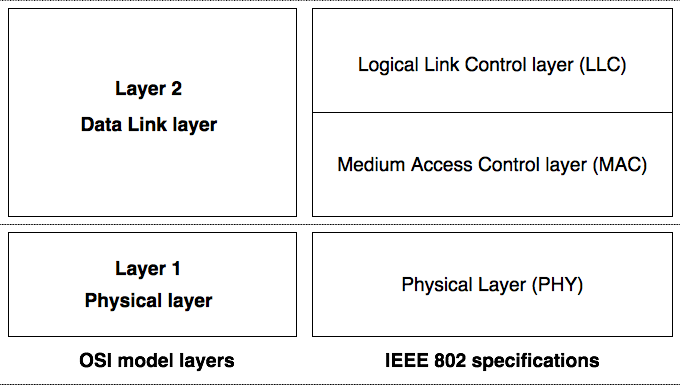
\includegraphics[scale=0.45]{img/osivs80211.png}
  \caption[OSI model layers vs IEEE~802 specification layers]{OSI model layers vs IEEE~802 specification layers.}
  \label{fig:layers}
\end{figure}

Wi-Fi networks, as other wireless technologies, use radio waves to send data over the air. A device that is used to send out a wireless signal is called transmitter. A device which can pick up that wireless signal and understands the information is called a receiver. A transceiver is a device that has both, a transmitter and a receiver. Different wireless technologies vary in used frequency and a type of modulation. Therefore, a device can only understand a specific wireless signal. The 802.11 standard provides several distinct radio frequencies ranges for use in Wi-Fi communication. In most countries, including European, it commonly operates in two frequency ranges: 2.4\,GHz and 5\,GHz bands. These bands are part of the \gls{ism} radio band, which is reserved internationally. Usage of these frequencies unlike others does not require a government license.

The 2.4\,GHz band is the most widely used of the bands available for Wi-Fi (used by 802.11b, g, n amendments). On one hand, devices operating on this band are cheaper to be manufactured than the ones used on the higher frequency. Besides, it is determined by physical laws that its signal, at the lower frequency, more easily penetrates through physical obstacles. On the other hand, there are significantly more devices using it. Thus, it is more prone to interference. The 5\,GHz band (used in standards 802.11a and ac) is considerably faster at short distances without obstacles. But the devices using this frequency are more expensive, and many do not support this option at all.

Each range is split into plenty of channels. Devices must be set to the the same channel to be able to communicate with each other. Countries apply different regulations to the legal channels, number of users and maximum power levels within these frequency ranges. Band 2.4\,GHz is given between 2,412 and 2,484\,GHz, which is divided into 14 independent channels after 5\,MHz steps. The fourteenth channel is an exception with a gap of 12\,MHz from the previous thirteenth one.

Wi-Fi communication requires a channel width of 20\,MHz to operate. Therefore, to avoid the interference between them, there can be only three running networks next to each other. The convention is to use the channels 1, 6 and 11 to avoid interference at the point of transmission. In Europe, the usage of the fourteenth channel is forbidden. The overlapping channels of the 2.4\,GHz band are illustrated in Figure~\ref{fig:channels}. The range of the 5\,GHz band is significantly higher. There are 19 available channels at this band in Europe. The first 8 for indoor usage and another 11 for outdoors. Channels in 5\,GHz band, are further away from each other (20\,MHz gaps). Hence, every device has its channel, and the signal does not interfere with others. The Access Points use the channels for regulation of the traffic.

\begin{figure}[h!]
  \centering
  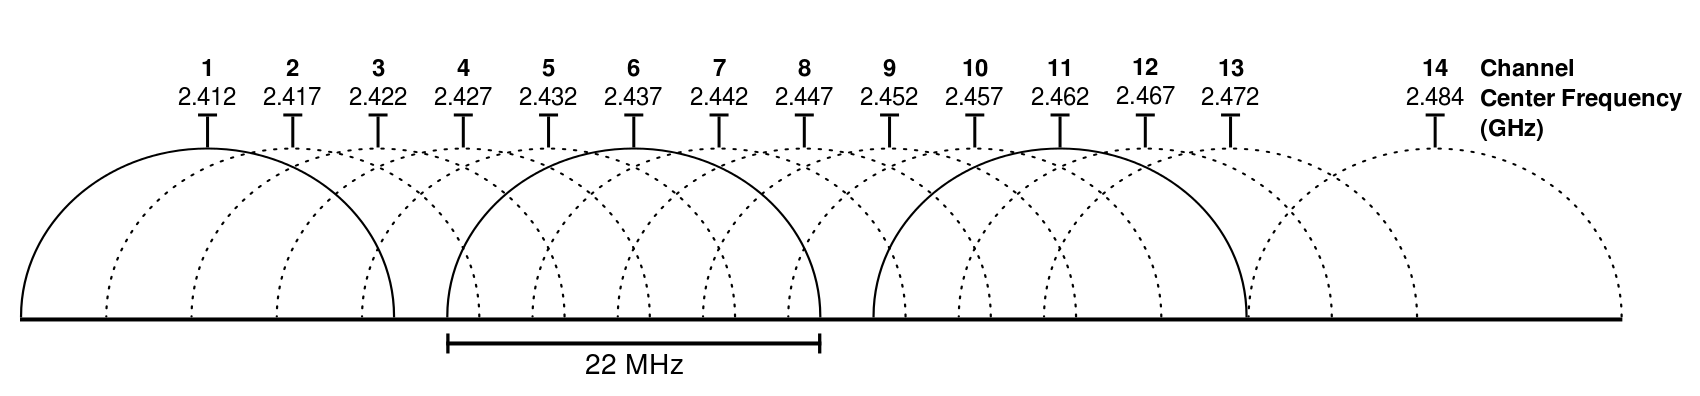
\includegraphics[scale=0.21]{img/2_4_GHz_Wi-Fi_channels.png}
  \caption[Graphical representation of 2.4\,GHz band channels overlapping]{Graphical representation of 2.4\,GHz band channels overlapping, figure taken from ~\cite{wi-finigel_2017}.}
  \label{fig:channels}
\end{figure}

The area where the wireless network is accessible to users is called a hotspot. When a group of wireless devices is operating with the same network parameters, it is called a service set. \gls{bss} is a group of devices running with the same MAC characteristics (radio frequency, modulation scheme, etc.). \gls{ess} is a set of logical units of one or more basic service sets on the same logical network segment (IP subnet, VLAN, etc.). A system interconnecting a set of BSSs and LANs to ESS is called \gls{ds}. Basic service sets are identified by \glspl{bssid} (48-bit label that conforms to MAC address convention) and Logical networks are identified by \glspl{ssid}. The SSID is commonly called a network name.

A Wi-Fi \gls{sta} is any addressable unit in a wireless network. The station can have one of three roles in a network. The networks are then built out of combinations of devices operating in these different modes. The first is an \gls{ap}. It is a networking hardware device that connects the Wi-Fi network to a wired network. This device creates a wireless local area network and devices on the network than communicate with this device to access the other networks or to communicate with each other. These connected devices are called clients or non-AP stations. Any laptop, mobile device or IoT device able to connect to a Wi-Fi network can be a client. The third possible device role is the ad-hoc node. This node is a device at the ad-hoc wireless network. The ad-hoc networks are the opposite of the managed (infrastructure) wireless networks, which are based on the AP and clients connected to it. It is decentralized, and every node participates in routing by forwarding data for other nodes.

The presence of a \gls{wnic} gives a device the ability to connect to a Wi-Fi network. It is a hardware component that connects to a wireless radio-based computer network and uses an antenna to communicate via microwave radiation. A WNIC in a desktop computer is traditionally connected using the PCI bus. Most of the laptops have a wireless network interface built into the motherboard. Another connectivity option is by external WNIC usually connected by USB. The WNIC can operate in two modes: infrastructure, which needs an access point, or ad-hoc mode, formed by ad-hoc nodes (without the need of AP). The WNIC specification usually consists of three crucial information: wireless data transfer rates (speed measured in Mbit/s), wireless transmitted power (measured in milliwatts or dBm) and supported wireless network standards. 

The WNIC, as others embedded systems, is on its lowest level controlled by firmware. This small piece of software stored in the Read Only Memory decides how the packets are handled and send. To be able to use WNIC in any operating system a user needs a driver. The driver is OS dependent since it is the software communicating between the OS and the WNIC. The chipset of the WNIC, its firmware and the driver used decides how the device handles packets received in the network.

The other important aspect of the wireless network is its range. It is given by the standard used, the power of the transmitter (and a type of an antenna), the nature of physical obstructions and radio interference in the surrounding area. The typical range of Wi-Fi is in several up to several tens of meters. It is typically higher outdoors because there are less physical obstacles.  
\section{Development and Certification}
   
The initial standard of this family, the IEEE~802.11-1997, was released in~1997 and is obsolete~\cite{GA05}. After publication of the initial document, customers were not satisfied with the degree of compatibility between devices of different vendors. This feedback from customers gave impetus to establish a certification program. For this purpose, the \gls{weca} was founded in 1999~\cite{HI10}. This alliance started the certification program and founded the trademark Wi-Fi. The certification program had a significant market impact. In 2003, the WECA was renamed to \gls{wfa}~\cite{HI10}, as we know it today. 

Because of the tremendous success in the market and the perceived shortcomings, the base 802.11 standard provided has been improved and expanded over the years. Additional amendments are distinguished by different letter suffixes (for example, 802.11a, 802.11i, 802.11w, etc.). Nowadays, there are many maintenance changes and amendments to the original standard. Some of the documents contain improvements to the previous ones regarding faster theoretical speed, extended range, security improvements, and lower power consumption. Others are offshoots of the base standard and serve a particular purpose (for example, 802.11i authentication and encryption, 802.11e \gls{qos}, 802.11w protected management frames, etc.). The goal is for all the 802.11 series of standards to be compatible at the Medium Access Control or Data Link layer. The document and project title, the year of approval and brief content of the significant documents are listed in Appendix~\ref{app:802.11}. The amendments defining protocols and handshakes vulnerable to the KRACK attack are listed below:

\begin{description}
\item [802.11i (2004)] Document deals with authentication and encryption. Its partial implementation is called WPA, and full is called WPA2. It defines the 4-way handshake, the PeerKey handshake, and the group Key handshake~\cite{ieee802.11i_2004}, all vulnerable to the KRACK attacks~\cite{VA17}. These handshakes are further discussed in Section~\ref{sec:security}.

\item [802.11r (2008)] It is also called Fast BSS Transition (or fast roaming). It describes technology to permit continuous connectivity aboard wireless devices in motion. The Fast BSS Transition handshake is also vulnerable to the KRACK attacks~\cite{VA17}. Thus, it will also be explained further in section~\ref{sec:security}. This standard also slightly extends the 4-way handshake and provides a particular state machine of the supplicant~\cite{ieee802.11r_2008}.

\item[802.11v (2011)] Deals with \gls{wnm} and device configuration. This amendment defines a WNM-Sleep mode. In~\cite{VA_ccs2018}, the author of the KRACK attack describes a way how to abuse WNM-Sleep response frames to trigger key reinstallation. 

\item[802.11z (2012)] Defines mechanism called \gls{tdls}. This mechanism enables a user to directly transfer data between two Wi-Fi clients that are part of the same Wi-Fi network. The TDLS PeerKey handshake is defined for this purpose and is also vulnerable to the KRACK attacks~\cite{VA_ccs2018} and will be further discussed in section~\ref{sec:security}.

\item[802.11ai (2016)] The document provides \gls{fils} methods to enhance end-user experience in dense environments. This function enables a wireless LAN client to achieve a secure link setup within 100\,ms. The FILS handshake is also vulnerable to the KRACK attack~\cite{VA_ccs2018}. Thus, it will be further discussed in the section~\ref{sec:security}.
\end{description}

As a basis for defining the basic concepts, available services and formats of frames, the IEEE~802.11-2016~\cite{revision2016} standard was used. According to the official IEEE~802.11 working group project timeline~\cite{ie18_timeline}, it is the latest published standard, including revisions defined in prior published amendments.

The IEEE does not test devices for compliance with their standards. The Wi-Fi Alliance does the only internationally-recognized certification program. This certification program ensures that products have met industry-agreed standards for interoperability, security, and a range of application-specific protocols. The program also provides a seal of approval that the certified products are backward-compatible with older published standards of the family.

\section{Establishing Communication}

There are two ways how the client can find out about the existing WiFi networks in a range:

\begin{itemize}
\item \textbf{Actively} The client sends a Probe Request on some channel and waits for a Probe Response from any access point. Inside response frames are network parameters (such as the SSID name networks or supported transfer rates and standards). Based on the obtained information, the client can initiate a network connection. The client sends requests periodically on all channels, to detect networks across the band.
\item \textbf{Passively} Access points send Beacon frame periodically with information about the network on the channel they are set to. The content of such a frame is similar to Probe Response. The client passively waits for such frames to capture network information across the band.
\end{itemize}

\subsection{Authentication and Association}

Before a client is allowed to communicate via an AP, it has to become authenticated and associated with the AP. In Wi-Fi networks, the process of authentication is used instead of the wired media physical connection. After authentication, the node has to be associated with an AP. Every node can be associated with no more than one AP, while an AP might be associated with many nodes at the same time. This way it can be unambiguously determined where to send the data specified for a specific node. When using WPA or WPA2 protocols, the system at first uses Open System Authentication, which allows any device to authenticate. The real authentication is performed later during the 4-way handshake. The process of establishing the IEEE~802.11 association is shown in Figure~\ref{fig:association}.

\begin{figure}[h!]
  \centering
  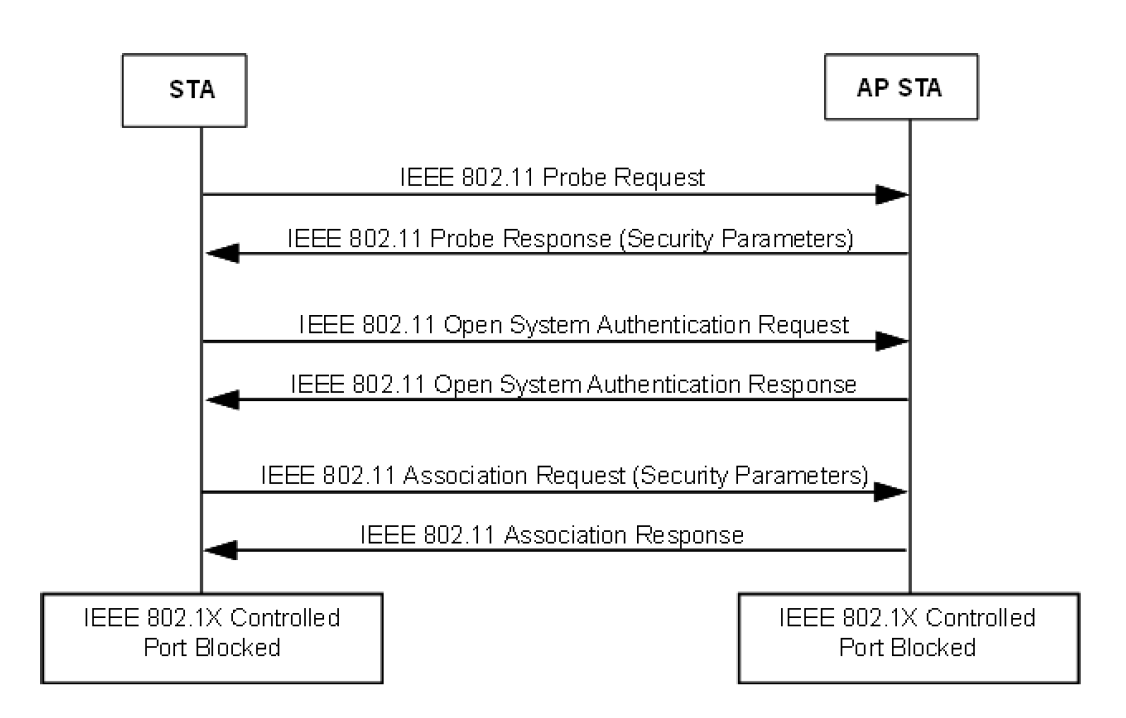
\includegraphics[scale=0.7]{img/authentication_association.png}
  \caption[Process of establishing the IEEE~802.11 association]{Process of establishing the IEEE~802.11 association, figure taken from ~\cite{ieee802.11i_2004}.}
  \label{fig:association}
\end{figure}

After this process is completed, there follows an optional 802.1x authentication process. This process is habitually used in enterprise and campus networks. After that, the 4-way handshake is performed to derive fresh session keys. The one for the unicast traffic is called \gls{ptk}, while the one for multicast or broadcast traffic is called \gls{gtk}. These keys are then used by a data-confidentiality and integrity protocol to encrypt data frames. 

\subsection{The 4-way Handshake}
\label{sub:fourWayHandshake}
The 4-way handshake is defined in the IEEE~802.11i amendment~\cite{ieee802.11i_2004}. According to the standard, during this handshake, a client is called a supplicant, and an AP is called an authenticator.

This handshake provides authentication based on the \gls{pmk}. In personal networks, the PMK is based on the pre-shared key, which is the password to the network. While in enterprise networks it is negotiated using 802.1x authentication stage. After authentication, the pairwise transient key (PTK) is derived. Concretely from the PMK, the authenticator nonce (ANonce), the supplicant nonce (SNonce) and the MAC addresses of both the AP and the client. The handshake is also used to transport the group temporal key (GTK) from the authenticator (the AP) to the supplicant (the client). When the GTK is transported, it is saved in the key data field, thus, encrypted using the PTK. The handshake uses EAPOL-Key frames. Their form will be shown in more detail in Subsection~\ref{sub:eapolKeyFrames}. The authenticity of each message except the first one is protected using \gls{mic}. The MIC is calculated using the subkey of the PTK called KCK. Every message also contains a replay counter. When the authenticator is sending a message, it always increments the replay counter, and the supplicant is replying to this message with the same replay counter.
The 4-way handshake takes place in four steps:

\begin{figure}[h!]
  \centering
  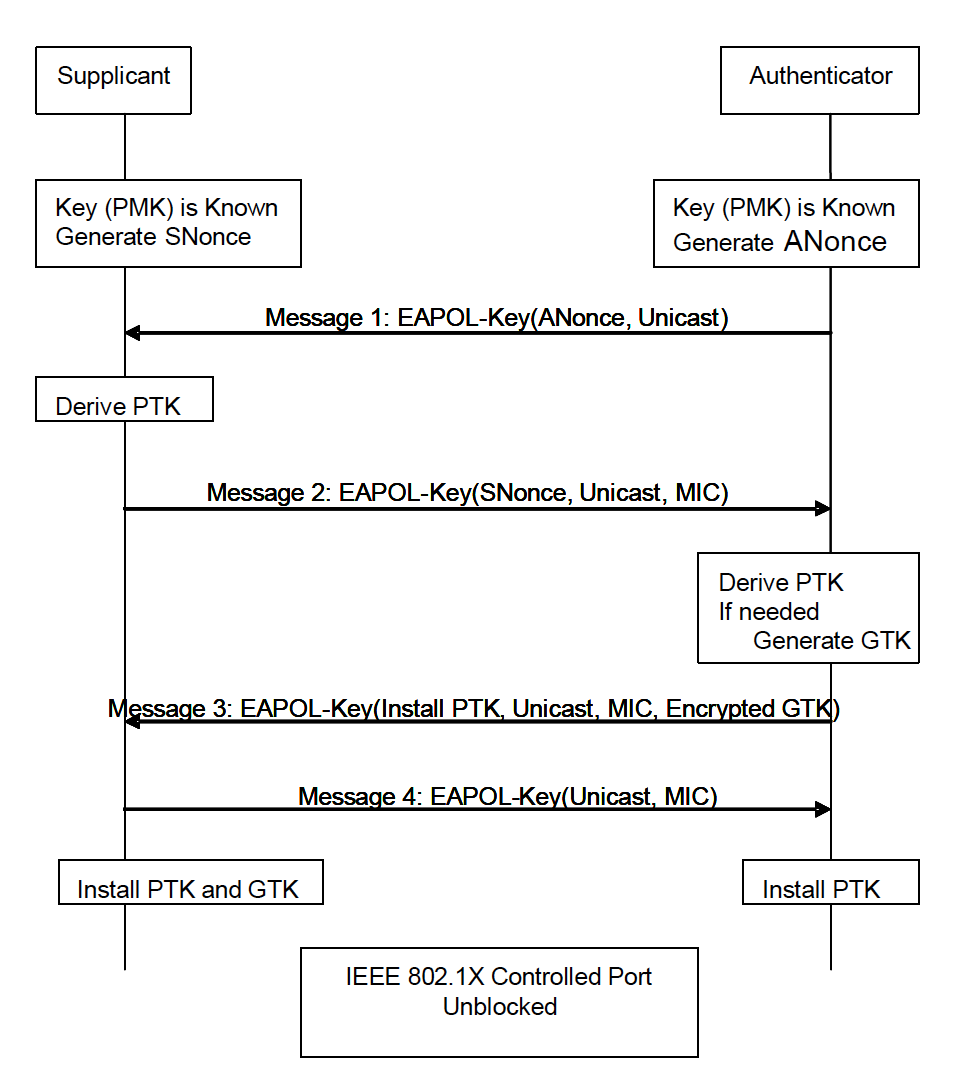
\includegraphics[scale=0.7]{img/4_way.png}
  \caption[The 4-way handshake]{The 4-way handshake, the figure was taken from~\cite{ieee802.11i_2004}.}
  \label{fig: 4_way_handshake}
\end{figure}

\begin{enumerate}
    \item At first, the authenticator sends an EAPOL-Key frame \textit{message~1}. This message contains random generated ANonce and has the replay counter of $r$.
    \item Then, the supplicant derives a PTK from ANonce and SNonce and sends an EAPOL-Key frame \textit{message~2} containing SNonce. This message also contains information from the (Re)Association Request frame about pairwise and group cipher suites supported. Besides, it contains MIC and replay counter $r$.
    \item Now the authenticator derives PTK from ANonce and SNonce and validates the MIC in the received EAPOL-Key frame \textit{message~2}. After the validation, the authenticator sends an EAPOL-Key frame \textit{message~3} again containing the same ANonce as in \textit{message~1}. It also contains information from its Beacon or Probe Response messages about pairwise and group cipher suites supported. Besides, it contains MIC, information whether to install the temporal keys and the encapsulated GTK. The message contains replay counter $r+1$.
    \item Finally, the supplicant sends an EAPOL-Key frame \textit{message~4} to confirm that the temporal keys are successfully installed. This message also contains replay counter $r+1$.
\end{enumerate}

After completion of the 4-Way Handshake, the authenticator and supplicant have been mutually authenticated and can send encrypted general data traffic to each other. The diagram of the 4-way handshake is shown in Figure~\ref{fig: 4_way_handshake}.

When a new 4-way handshake is initialized, the messages of the handshake are encrypted by the already installed PTK. Also, the nonces of the authenticator and supplicant are refreshed, and a new PTK is negotiated.

\subsection{The Group Key Handshake}
The group key handshake is also defined in the amendment IEEE~802.11i~\cite{ieee802.11i_2004}. The authenticator uses this handshake to send a new GTK to the supplicant. It is done periodically; the period depends on settings of the AP. Also, the supplicant may trigger a group key handshake by sending an EAPOL-Key frame with the Request bit set to 1 and the type of the group Key bit. It can be done only after the 4-way handshake was successfully performed. Thus, all messages of the group key handshake are encrypted using the data-confidentiality protocol.

\begin{figure}[h!]
  \centering
  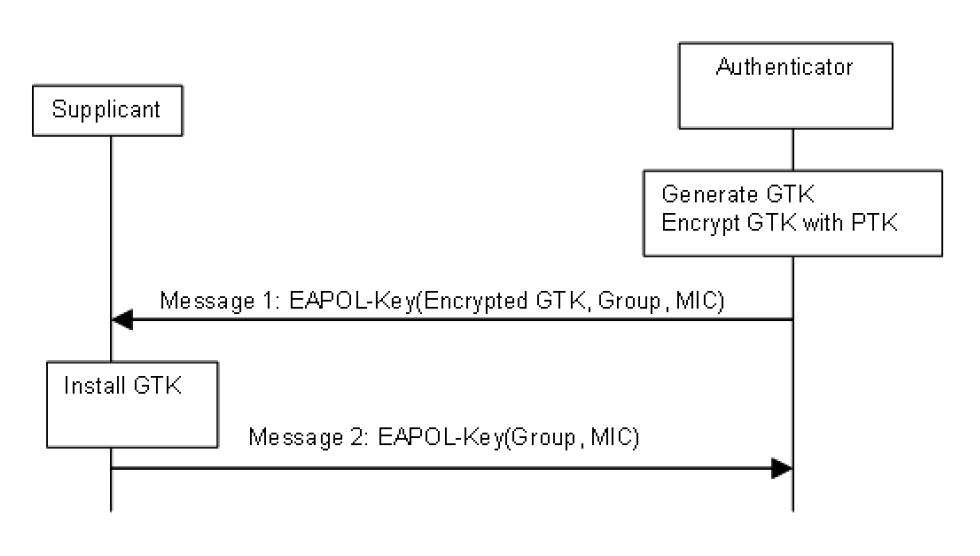
\includegraphics[scale=0.7]{img/groupKeyHandshake.png}
  \caption[The group key handshake]{The group key handshake, the figure was taken from~\cite{ieee802.11i_2004}.}
  \label{fig: group_key_handshake}
\end{figure}

The group key handshake takes place in two steps:
\begin{enumerate}
    \item The authenticator initiates the handshake by sending EAPOL-Key frame containing the GTK as \textit{message~1} with a new encapsulated GTK, along with the last sequence number used with the GTK (RSC). The GTK is, as in the 4-way handshake, stored in the Key data field, thus, it is encrypted using KEK.
    \item  On receiving the EAPOL-Key frame, the supplicant validates the MIC, decapsulates the GTK, and installs the GTK and the RSC. The supplicant then constructs and sends an EAPOL-Key frame \textit{message~2} in acknowledgment to the authenticator.
\end{enumerate}

There are two variants when the authenticator installs the group key. First is after sending \textit{message~1}, the second is after receiving \textit{message~2} from all the supplicants. The specific variant used by a device depends on the implementation, this is further described in~\cite{VA_ccs2017}.
When a client sends a group frame (broadcast or multicast), it is first sent to the AP as a unicast frame, and then the AP encrypts it using group key and sends it to all clients. The diagram of the group key handshake is in Figure~\ref{fig: group_key_handshake}.

\section{Security}
\label{sec:security}

In the base 802.11 standard published in 1997, there was defined a security algorithm for data encryption. This algorithm was called \gls{wep}. Due to the absence of the certification program at the beginning, its usage was only optional. Shortly after its release, already in 2001, the protocol was broken~\cite{Cam-Winget03, finalNailWEP, VA17, MEKHAZNIA_2015}. In response, the IEEE developed the 802.11i standard to upgrade the encryption algorithm. In this standard, the protocols \gls{wpa} and \gls{wpa2} were defined along with the 4-way and group key handshakes~\cite{ieee802.11i_2004}. The WPA protocol is based on \gls{tkip}, a robust encryption algorithm built around WEP. This algorithm was able to run on the same hardware as the original WEP. Thanks to this, only updating firmware was necessary to upgrade from WEP to WPA. It was certified by Wi-Fi Alliance based on a draft version of the 802.11i amendment which was still in development during that time. The protocol was meant as a temporary compensation before the amendment was finished and the Wi-Fi Alliance later deprecated the TKIP for the insufficient level of security~\cite{TKIP_deprecated}. The full implementation of the 802.11i standard is certified as WPA2, and it is built on the \gls{ccmp} of the \gls{aes} algorithm. Due to the higher computational complexity of the \mbox{(AES-)CCMP} encryption, it was necessary to replace previously used hardware to use WPA2. The data-confidentiality and integrity protocol used is the main difference between WPA and WPA2. Otherwise, they are very similar to each other, and both use the 4-way handshake, either in personal or enterprise networks~\cite{ieee802.11i_2004}. Additional data-confidentiality and integrity protocol was defined in amendment 802.11ad published in 2012. It is called \gls{gcmp}~\cite{IEEE802_11ad}.

In January 2018, the Wi-Fi Alliance announced the release of the WPA3 with several security improvements over WPA2~\cite{wpa3}. Unfortunately, WPA3 does not provide users with absolute assurance that they will not be vulnerable to KRACK attacks. Although the WPA3 protocol provides a new Dragonfly handshake, it will be used in combination with the 4-way handshake~\cite{vanhoef_2018_WPA3}. Therefore, the vulnerability of the WPA3 certified products will again depend on the specific implementation of the 4-way handshake. 

\subsection{Data Confidentiality and Integrity Protocols}

Nowadays, there are three data confidentiality and integrity protocols in use (we exclude the deprecated WEP): TKIP, CCMP, and GCMP. These protocols are used for encryption of data frames. There is also an algorithm used for authentication (not encryption) of group-addressed management frames called \gls{bip} but we will not deal with it in this work. The implementation of the CCMP is mandatory in all WPA2 certified devices. It also optionally supports TKIP but only for backward compatibility reasons. The WPA is exactly the other way; it mandates support for TKIP and optionally supports CCMP. 

\begin{figure}[h!]
  \centering
  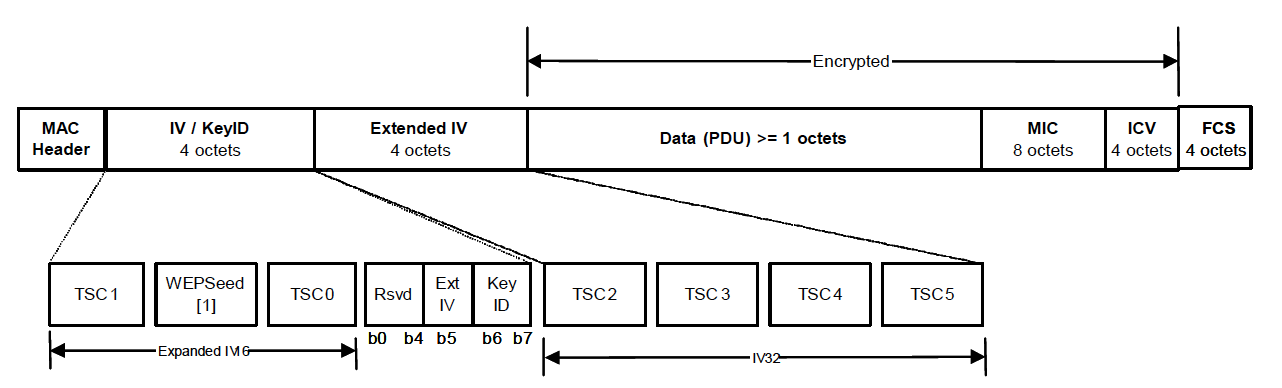
\includegraphics[scale=0.6]{img/TKIP_MPDU.png}
  \caption[Expanded TKIP MPDU]{Expanded TKIP MPDU, figure taken from~\cite{ieee802.11i_2004}.}
  \label{fig: TKIP_MPDU}
\end{figure}

The TKIP was designed to be able to operate on the machines which used to use WEP and should only be used when communicating with devices that are unable or not configured for encryption using CCMP or GCMP. It uses the same cipher as older WEP, the RC4. When using TKIP, the \gls{tk} which is part of the session key (PTK) is further split into a 128-bit encryption key and two 64-bit MICs. One is used for communication from an AP to a client and the second one in reverse. MIC provides a defense against forgery attacks. TKIP uses per-frame \gls{tsc}, which is incremented after transmitting a frame and initialized to 1 when installing the TK. Besides, it is used as a replay counter. The WEP seed, which is the keystream used to encrypt the data and MIC, is a mix of the 128-bit encryption key, the sender MAC address, and an incremental TSC. This TSC is by Vanhoef denoted as nonce~\cite{VA_ccs2017}. Message authenticity is provided by the Michael algorithm. The expanded \gls{mpdu} using TKIP is shown in Figure~\ref{fig: TKIP_MPDU}. 

\begin{figure}[h!]
  \centering
  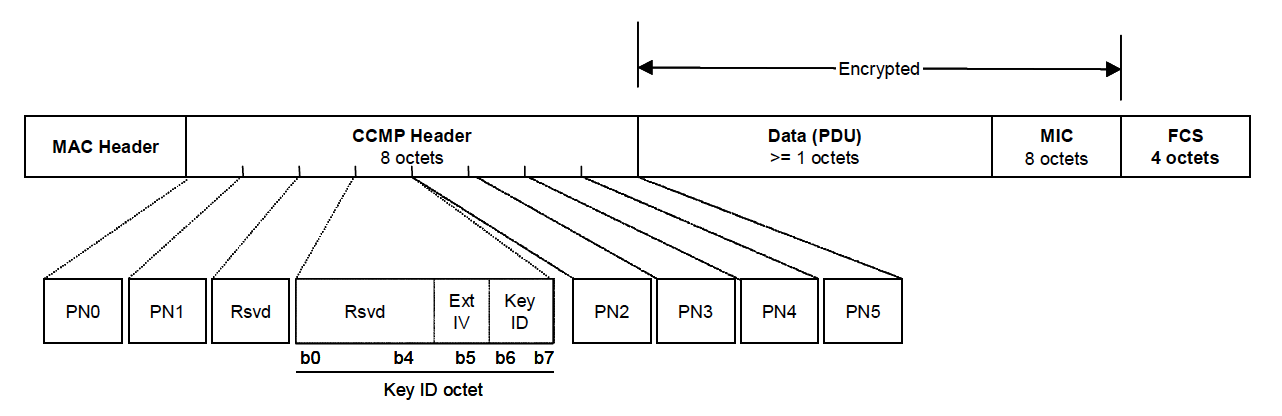
\includegraphics[scale=0.6]{img/CCMP_MDPU.png}
  \caption[Expanded CCMP MPDU]{Expanded CCMP MPDU, figure taken from~\cite{ieee802.11i_2004}.}
  \label{fig: CCMP_MPDU}
\end{figure} 

The CCMP is based on the Counter with \gls{ccm} mode of the AES encryption algorithm. The nonce of the CCMP is the concatenation of the sender MAC address, a 48-bit \gls{pn}, and some additional flags derived from the transmitted frame. According to standard, the encryption algorithm is secure, as long as, the nonce is used only once for the same key. This nonce is by Vanhoef called the \gls{iv}, and the packet number is what he calls the nonce~\cite{VA_ccs2017}. The number is also used as a replay counter by the receiver, and it is initialized to 0 when installing the temporal key. The expanded MPDU when using CCMP is shown in Figure~\ref{fig: CCMP_MPDU}.

\begin{figure}[h!]
  \centering
  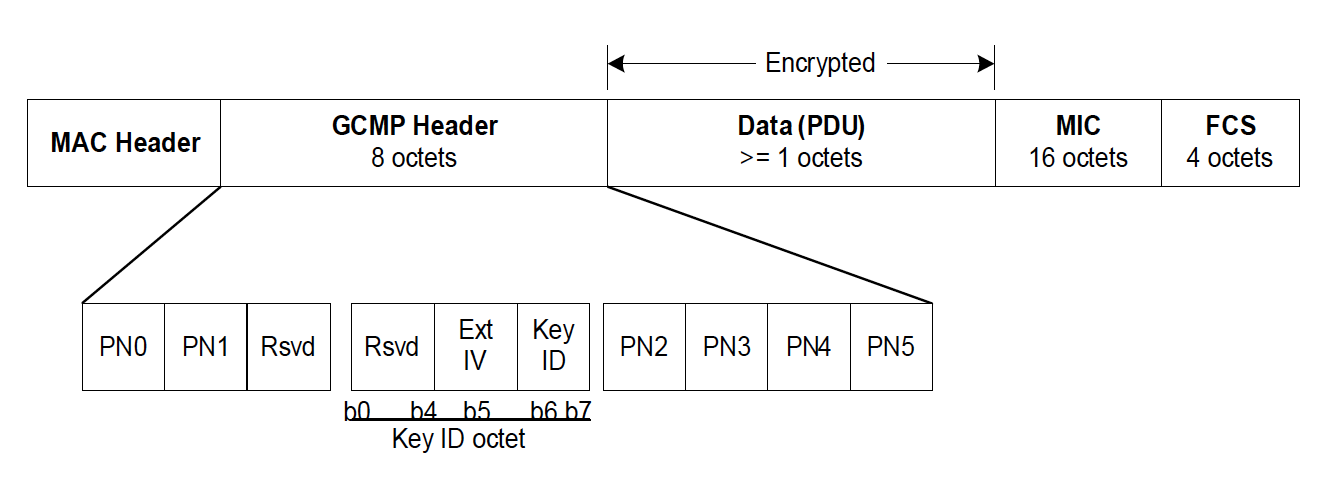
\includegraphics[scale=0.55]{img/GCMP_MPDU.png}
  \caption[Expanded GCMP MPDU]{Expanded GCMP MPDU, figure taken from~\cite{IEEE802_11ad}.}
  \label{fig: GCMP_MPDU}
\end{figure}

The GCMP is based on the AES cipher with Galois/Counter Mode. Besides, it uses GMAC for authentication and integrity. As the CCMP, GCM requires a fresh temporal key for every session and a unique nonce value for each frame protected by a given temporal key. Similarly, as the CCMP, the GCMP uses a nonce that is a concatenation of the sender MAC address and a 48-bit packet number. Also, the PN is used as a replay counter by the receiver, and it is initialized to 0 when installing the temporal key. The packet number is what is called nonce by Vanhoef~\cite{VA_ccs2017}. The expanded MPDU when using GCMP is shown in Figure~\ref{fig: GCMP_MPDU}.

\section{Other Vulnerable Handshakes}
This section briefly introduces other handshakes that are vulnerable to the KRACK attack.

\subsection{The PeerKey Handshake}
This handshake was defined in IEEE~802.11-2016~\cite{revision2016} and is used to provide data confidentiality between the two STAs. The handshake consists of two phases. First, the SMK handshake is performed to achieve \gls{stsl} master key security association (SMKSA), which is then installed in both the STAs. This message exchange goes via the AP and is protected using the PTK. The second phase is the 4-way STK handshake. This handshake runs as well as the standard 4-way handshake, except the initial authentication is done using the installed SMKSA, and as a result of this, the STKSA gets installed in both the STAs. This handshake is very rarely used, and in an IEEE report from January 2018~\cite{IEEEP802.11}, it is marked obsolete. Its deprecation is planned in the future standard revision. Since the vulnerable phase of this handshake is the 4-way handshake which runs in the same manner as the original 4-way handshake, the diagram of this handshake will be omitted from the description. 

\subsection{\gls{ft} Handshake}
This handshake is defined in the amendment IEEE~802.11r-2008~\cite{ieee802.11r_2008}. It is used when the client is roaming between APs of the same network. It reduces time by setting up security and QoS parameters before reassociation to a new AP, and thus, speeds up the time-critical reassociation process. This handshake is important because it is the only handshake vulnerable on the side of the AP. If the AP does not support this standard, it cannot be vulnerable to the KRACK attacks. 

\begin{figure}[h!]
  \centering
  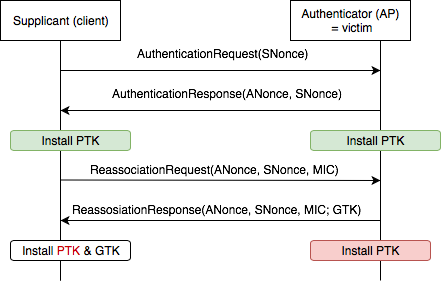
\includegraphics[scale=0.7]{img/FThandshake.png}
  \caption[The Fast BSS Transition handshake]{The Fast BSS Transition handshake with denoted installation of the PTK defined in standard (green --- not vulnerable) and found in specific implementations by Vanhoef (red --- vulnerable).}
  \label{fig:ftHandshake}
\end{figure}

This handshake is done when the client is already connected to the network. Therefore, it relies on master keys derived during the previous connection. Functionally, it performs the same operations as the 4-way handshake but using the Authentication and (Re)Association frames. Unlike the 4-way handshake, it is initialized by the supplicant, not the authenticator. But the messages have the same purpose. The first two messages serve as authentication, the other two transport the GTK to the client. The third and fourth message is protected by MIC, but none of the messages contain a replay counter. It only relies on random ANonce and SNonce values which identify the handshake (the authenticator and the supplicant generate random nonce value for each handshake).  

According to the standard, this handshake is not vulnerable to the KRACK attack, because the PTK must be installed after the authentication response is sent or received. This would be after the first two messages of the handshake, as you can see in Figure~\ref{fig:ftHandshake}, where it is colored green. On the contrary, Vanhoef found by testing specific devices, that they install the PTK after the whole handshake. It is further discussed in~\cite{VA_ccs2017}. This is colored red in the Figure~\ref{fig:ftHandshake}.

\subsection{\gls{fils} Handshake}

The FILS handshake was published in the IEEE~802.11ai-2016 amendment~\cite{IEEE802_11ai_2016}. This protocol serves to establish a secure connection to an AP and simultaneously initialize higher layer protocols.

The FILS authentication can be performed by public or shared secret key. When using a shared secret key, it could be either PMK or \gls{rrk} which is derived during the 802.1x. The handshake is again very similar to the 4-way handshake, but it uses Authentication Request and Response frames, following by (Re)Association Request and Response frames. The authentication frames also contain EAP-initiate/Re-auth packet which is defined in RFC 6696~\cite{RFC6696}. The (Re)Association Request and Response again serve to confirm negotiation of the same PTK but can additionally include a DHCP request and response. The messages in the handshake do not include a replay counter. 

\subsection{\gls{tpk} Handshake}
The TPK handshake is defined in standard  IEEE~802.11z-2010~\cite{IEEE_802_11z_2010}. This handshake is used to establish a direct link secure tunnel between two STAs, an initiator, which initiates the link established, and a responder. Establishing of the tunnel runs via an AP. For that purpose, both the initiator and the responder have to have a secure link between them and the AP established at first. Assuming they have it, the TPK 3-way handshake can proceed. First, the initiator sends TDLS Setup Request frame with TPK handshake \textit{message~1} included. The responder sends TDLS Setup Response frame with TPK handshake \textit{message~2}. When the initiator receives the message, he or she installs the TPK and as a response, sends the TDLS Setup Confirm frame with TPK handshake \textit{message~3}. The responder installs the TPK after receiving the third message of the handshake. When the direct link is established, they become TDLS peer STAs and can communicate directly with each other in a secure manner. This connection is used to directly stream data between devices, for example, between a PC and a printer or for storing data to external storage. The transmitted information between these devices might be easily confidential. The standard does not provide any state machine of the handshake, and this thesis is not going to examine this handshake further in more detail. Thus, the diagram will be omitted from description.

\section{MAC Frames}
\label{sec: mac_frames}
Communication on the link layer takes place using frames in the following format (defined according IEEE~802.11-2016~\cite{revision2016}).

\subsection{General 802.11 Frame}
A general 802.11 frame always consists of three following basic components:

\begin{enumerate}[\hspace{2cm}(a)]
    \item A \textit{MAC header}
    \item A variable-length \textit{frame body}
    \item A \textit{\gls{fcs}}
\end{enumerate}

The format consists of a set of fields that occur in a fixed order in all frames. The Figure~\ref{fig:frameFormat} depicts the general MAC frame format. The first three fields (Frame Control, Duration/ID, and Address 1) and the last field (FCS) form the minimal frame format. These fields are present in all frames which includes reserved types and subtypes. Other fields and Frame Body are present only in certain frame types and subtypes.

\begin{figure}[h!]
  \centering
  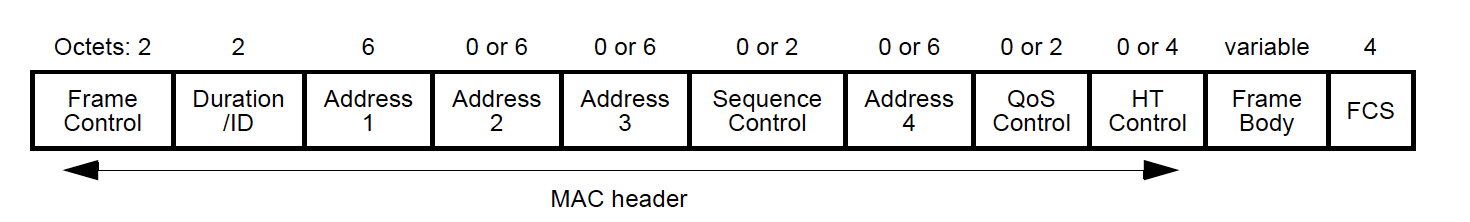
\includegraphics[scale=0.5]{img/MAC_frame_format.png}
  \caption[General MAC frame format]{General MAC frame format, figure taken from ~\cite{revision2016}.}
  \label{fig:frameFormat}
\end{figure}

The first three subfields of the Frame Control field, Protocol Version, Type, and Subtype, are the same for all types and subtypes of the frame. The remaining subfields of the Frame Control field depend on the combination of the Type and Subtype subfields. The structure of the frame Control field can be seen in Figure~\ref{fig:frameControl}. This holds for all frames except the frame of subtype Control Frame extension, which is not relevant to this work.

\begin{figure}[h!]
  \centering
  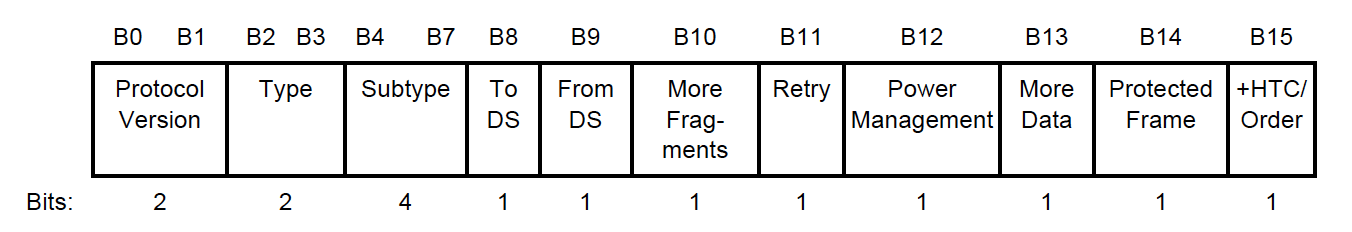
\includegraphics[scale=0.55]{img/Frame_Control_Subfield.png}
  \caption[Frame Control field structure]{Frame Control field structure except for the Control Frame Extension subtype, figure taken from ~\cite{revision2016}.}
  \label{fig:frameControl}
\end{figure}

The Frame Control field contains flags about type and subtype of the frame. Additionally, it indicates the direction of the communication, if it is from the client to the \gls{ds} or vice versa. Other flags designate if the packet was split into multiple frames for transmission or if it was retransmitted. Additionally, there are flags helping with power management of the stations. When a station is going to the "Power Save Mode", it notifies other devices about being in this mode by sending a Null Data frame with only Power Management bit set to 1. According to Vanhoef~\cite{VA18}, the WNM-Sleep response frames, used by an AP to confirm or disprove the client's WNM-Sleep Request (frame indicating that client wants to enter sleep mode), can be abused to trigger key reinstallations. Another subfield then designates if the AP has buffered some frames for this device in the low power consumption mode. The important subfield regarding encryption is the Protected Frame flag. It indicates if the frame body was encrypted by an encryption algorithm, such as WEP, WPA, or WPA2.

An 802.11 frame can have up to four address fields. According to the type and subtype of the frame, the frame fields Address 1 to Address 4 contain a combination of the following addresses:

\begin{description}
\item \textbf{\gls{bssid}} This is an identifier of a set of devices which can communicate with each other in a wireless network. In infrastructure networks, it is the address of an AP. 
\item \textbf{\gls{sa}} Source address of the device which created and sent the frame to the network. 
\item \textbf{\gls{da}} Destination address of the device which is supposed to receive the frame.
\item \textbf{\gls{ta}} Address of the device which sent the frame to the network.
\item \textbf{\gls{ra}} Address of the next device in the network which will receive the frame.
\end{description}

The address can be individual, designating a specific station on the network, or group address. The group address then can be either multicast-group address or broadcast address. Multicast address brings together a group of logically related STAs. Broadcast is predefined group address that always denoted the set of all STAs on a given LAN. 

Most of the frames (depends on type) have the Sequence Control field. This field is a two-byte section consisting of Sequence Number of the frame and the Fragment Number field indicating the number of each fragment.

Each frame has the \gls{fcs}. It allows for integrity check of retrieved frames. Before sending a frame, the FCS is calculated and appended as the last four bytes. A receiving station calculates the FCS and checks if they are equal with the one received. This way, the station checks that the frame was not malformed during transmission.

In the 802.11 standard, three major frame types exist: 

\begin{itemize}
\item \textbf{Control Frames (Type bits = 01)}
Control frames facilitate the exchange of data and management frames between stations. These frames, unlike other types, does not contain frame body. For example, subtype RTS is the request-to-send frame, and CTS is the clear-to-send frame which is often sent as a response to RTS. A special frame is ACK, which is sent as an acknowledge to confirm reception of a frame.

\item \textbf{Management Frames (Type bits = 00)}
802.11 management frames enable stations to establish and maintain communications. These frames are used to support authentication, association, and synchronization. Some examples of these frames are Beacon frame, Probe Request, and Response, (Re)Association Request and Response,  which were already mentioned. The opposite to them is the Disassociation frame which is sent to terminate the association of a station and Deauthentication frame which is sent for terminating the authentication of a station. 

\item \textbf{Data Frames (Type bits = 10)}
Data frames carry higher-level protocol data in the frame body. The Address 1, Address 2, Address 3 and Sequence Control are present in all data frame subtypes. Data frames with a value of 1 in the QoS subfield of the Subtype subfield are collectively referred to as QoS Data frames. Each of these data subtypes contains QoS in their names, and this frame format is distinguished by the presence of a QoS Control field in the MAC header. EAPOL frame is also one of the QoS data frames, and its subtype EAPOL-Key frame is used in the 4-way, group key and PeerKey handshake. Its format will be further discussed in Section~\ref{sub:eapolKeyFrames}.
\end{itemize}

The table of existing subtypes is listed in Appendix~\ref{app:frameSubtypes}. The frames with the type field bits set to 11 are Reserved frames.

\subsection{EAPOL-Key Frames}
\label{sub:eapolKeyFrames}

An eapol-key frame is a type of an EAPOL frame used to exchange cryptographic keying information between supplicants and authenticators. The format of an EAPOL-Key frame is shown in Figure~\ref{fig:EAPOLKey}.

\begin{figure}[h!]
  \centering
  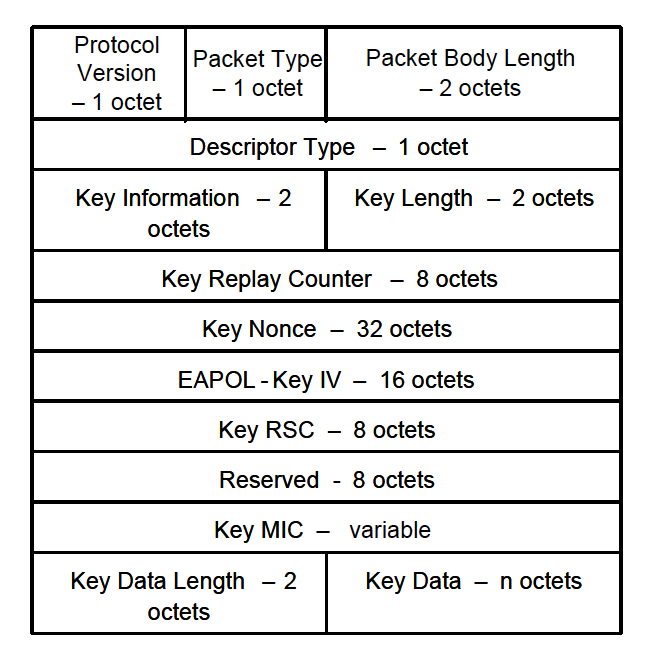
\includegraphics[scale=0.7]{img/EAPOL-Frame.png}
  \caption[EAPOL-Key frame structure]{EAPOL-Key frame structure, figure taken from ~\cite{revision2016}.}
  \label{fig:EAPOLKey}
\end{figure}

Important characteristics of the key are determined by flags which are stored in field Key Information. Its structure is shown in Figure~\ref{fig:KeyInformation} and its subfields are described below:

\begin{figure}[h!]
  \centering
  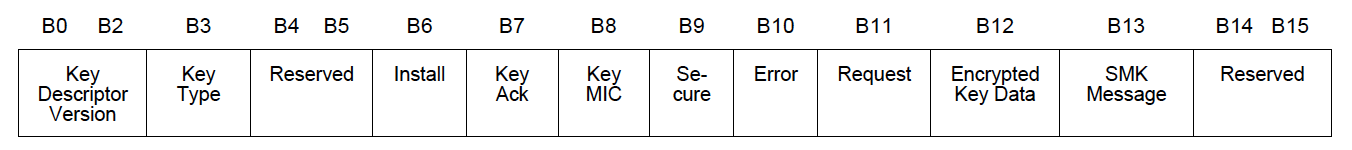
\includegraphics[scale=0.55]{img/KeyInformation.png}
  \caption[Key Information structure]{Key Information structure --- Bx designate individual bits, figure taken from ~\cite{revision2016}.}
  \label{fig:KeyInformation}
\end{figure}

\begin{description}
\item \textbf{Key type}: If set to 1, the frame is part of the 4-way handshake (deriving PTK). If not, it is part of the group key handshake (distributing GTK).
\item \textbf{Install}: Determines if the key should be installed by the receiving station or not.
\item \textbf{Key ack}: If set to 1, the message is from the authenticator, and so, it requires acknowledgment message. The acknowledgment message should use the same replay counter as this message.
\item \textbf{MIC}: Determines if the frame is protected by MIC or not. 
\item \textbf{Secure}: Both the authenticator and the supplicant set it to 1 when both the PTK \& GTK were sent (thus, the initial key exchange is completed).
\item \textbf{Request}: The supplicant sets it to 1 when it wants to initialize a new 4-way or group key handshake or in case of MIC check failure. The authenticator never sets it to 1.
\item \textbf{Encrypted Key Data}: It is set to 1 in case Key Data field is encrypted. This happens in the case when GTK or STK keys are present in the Key Data field.
\item \textbf{SMK message}: The flag specifies whether this EAPOL frame is part of an SMK handshake (the second phase of the PeerKey handshake).
\end{description}

The meaning of other relevant fields is as follows: 
\begin{description}
\item \textbf{Key Length}: This field determines the length of the PTK; it depends on the cipher used for encryption.
\item \textbf{Key Replay Counter}: It is set to 0 when PTK is installed. The authenticator increments it by 1 at each successive EAPOL-Key frame. The supplicant uses the same key replay counter in replays to the received frames.
\item \textbf{Key Nonce}: Contains ANonce (from the authenticator) or SNonce (from the supplicant).
\item \textbf{Key RSC}: Contains the received Receive Sequence Counter for the GTK being installed. 
\item \textbf{Key Data Length}: It determines the length of the Key data field. If its encryption is required, it contains the length after the encryption.
\item \textbf{Key Data}: This field is a variable-length field that is used to include any additional data required for the key exchange that is not included in the fields of the EAPOL-Key frame.
\end{description}

If any of the fields is not required in the message, it contains 0. If the EAPOL-Key frame does not have the required form, it is dropped.

